\documentclass[11pt,a4paper]{article}
\usepackage[margin=2.2cm]{geometry}
\usepackage{amsmath,amssymb,amsfonts}
\usepackage{hyperref}
\usepackage{booktabs}
\usepackage{graphicx}
\usepackage{xcolor}
\usepackage{enumitem}
\usepackage{float}
\usepackage{caption}
\usepackage{fancyhdr}

\hypersetup{
  colorlinks=true,
  linkcolor=blue!70!black,
  citecolor=blue!70!black,
  urlcolor=blue!70!black,
  pdftitle={Dark Energy from Secluded Majorana SIDM -- Supplementary Material},
  pdfauthor={Omer Pesach}
}

\newcommand{\Mpl}{M_{\mathrm{Pl}}}
\newcommand{\Ld}{\Lambda_d}
\newcommand{\meV}{\,\mathrm{meV}}
\newcommand{\GeV}{\,\mathrm{GeV}}
\newcommand{\MeV}{\,\mathrm{MeV}}
\newcommand{\kms}{\,\mathrm{km/s/Mpc}}

\pagestyle{fancy}
\fancyhf{}
\fancyhead[L]{\small Secluded Majorana SIDM --- Paper 2 Supplement}
\fancyhead[R]{\small O.~Pesach (2026)}
\fancyfoot[C]{\thepage}

\title{\textbf{Dark Energy from a Secluded Dark QCD Sector}\\[4pt]
\Large Quintessence, Dimensional Transmutation, and DESI DR2\\[8pt]
\large Supplementary Material \& Figures\\[4pt]
\normalsize Paper~2 of the Secluded Majorana SIDM Program}
\author{Omer Pesach\\[2pt]
\small ORCID: \href{https://orcid.org/0009-0004-8178-8131}{0009-0004-8178-8131}\\[2pt]
\small Contact: \texttt{omerpesach@gmail.com}}
\date{March 29, 2026}

\begin{document}
\maketitle
\thispagestyle{fancy}

%=====================================================================
\begin{abstract}
\noindent
This document accompanies the Zenodo data release for Paper~2 of the Secluded Majorana SIDM program.
We demonstrate that the CP-violating phase in a secluded Majorana self-interacting dark matter model
gives rise to a quintessence field---a dark pion $\sigma$ from SU(2)$_d$ confinement---whose
potential drives the current cosmic acceleration. The dark QCD confinement scale
$\Ld \approx 2\meV$ emerges via dimensional transmutation from $\alpha_d \sim 0.03$,
resolving the cosmological constant hierarchy without fine-tuning.
Including the leading multi-instanton correction
$V(\theta)=\Ld^4[(1-\cos\theta)+\varepsilon(1-\cos 2\theta)]$ with
$\varepsilon\approx -0.10\pm 0.03$, the model matches DESI DR2 BAO measurements
at the $1.1$--$1.4\sigma$ level across all seven redshift bins.
This supplement contains model description, key formulas, numerical results, and
publication-quality figures.

\medskip\noindent
\textbf{Related resources:}
\begin{itemize}[nosep]
  \item Paper~1 (SIDM sector): Zenodo DOI \href{https://doi.org/10.5281/zenodo.19225823}{10.5281/zenodo.19225823}
  \item GitHub: \url{https://github.com/0mp3s/dark-energy-T-breaking}
\end{itemize}
\end{abstract}

\tableofcontents
\newpage

%=====================================================================
\section{Overview of the Model}
\label{sec:model}
%=====================================================================

The model extends the secluded Majorana SIDM Lagrangian established in Paper~1
by promoting the CP-violating phase $\theta$ of the dark Yukawa coupling to a dynamical
pseudo-Nambu--Goldstone boson $\sigma$ (a dark pion) from SU(2)$_d$ confinement.

\subsection{SIDM Lagrangian (Paper~1)}

\begin{equation}\label{eq:lag}
\mathcal{L}_{\mathrm{SIDM}} = \tfrac{1}{2}\bar\chi(i\!\not\!\partial - m_\chi)\chi
+ \tfrac{1}{2}(\partial\phi)^2 - V_0(\phi)
- \tfrac{1}{2}\bar\chi\bigl(y_s + iy_p\gamma^5\bigr)\chi\,\phi
\end{equation}

\noindent
\textbf{MAP benchmark parameters} (from Paper~1's global fit to 13 astrophysical systems):
\begin{equation}
  m_\chi = 98.19\GeV, \quad m_\phi = 9.66\MeV, \quad \alpha_D = 3.274\times 10^{-3}
  \quad\Rightarrow\quad \Omega_\chi h^2 = 0.120
\end{equation}

\subsection{CP phase promotion}

\begin{equation}\label{eq:promotion}
  y_s + iy_p\gamma^5 \;\longrightarrow\; y\,e^{i\gamma^5\sigma/f}
  \;=\; y\cos\!\Bigl(\frac{\sigma}{f}\Bigr) + iy\sin\!\Bigl(\frac{\sigma}{f}\Bigr)\gamma^5
\end{equation}
where $f$ is the dark pion decay constant and $\sigma$ is the Goldstone of spontaneous chiral
symmetry breaking in SU(2)$_d$ with 3 Majorana quarks.

\subsection{Dark pion potential with higher harmonics}

The leading-order chiral Lagrangian gives $V=\Ld^4(1-\cos\theta)$.
Including the next-to-leading multi-instanton correction:

\begin{equation}\label{eq:potential}
  \boxed{V(\sigma) = \Ld^4\Bigl[(1 - \cos\theta) + \varepsilon(1 - \cos 2\theta)\Bigr],
  \qquad \theta \equiv \sigma/f}
\end{equation}

The second-harmonic coefficient $\varepsilon$ encodes the ratio of 2-instanton to 1-instanton
amplitudes. For $\varepsilon < 0$, the potential hilltop at $\theta = \pi$ is sharpened,
enabling a steeper equation-of-state evolution that matches DESI DR2.

%=====================================================================
\section{Dimensional Transmutation}
\label{sec:transmutation}
%=====================================================================

The dark confinement scale is generated by the SU(2)$_d$ RG running:

\begin{equation}\label{eq:transmutation}
  \Ld = \mu \cdot \exp\!\Bigl(-\frac{2\pi}{b_0\,\alpha_d(\mu)}\Bigr),
  \qquad b_0 = \frac{11 N_c - 2 N_f}{3} = \frac{11\times 2 - 2\times\tfrac{3}{2}}{3} = \frac{19}{3}
\end{equation}
for SU(2)$_d$ ($N_c = 2$) with $N_f = 3/2$ Dirac flavors (3 Majorana).

\medskip
\noindent
\textbf{Numerical evaluation:}
\begin{equation}
  \Ld = 98\GeV \times \exp\!\Bigl(-\frac{2\pi}{6.333 \times 0.031}\Bigr)
  \approx 2.0 \times 10^{-12}\GeV = 2\meV
\end{equation}

This trades the $10^{122}$ cosmological constant hierarchy for two unremarkable inputs:
\begin{enumerate}[nosep]
  \item A gauge coupling $\alpha_d \sim 0.03$ at $\mu = m_\chi$ (comparable to $\alpha_{\mathrm{EM}}$)
  \item A standard hierarchy $m_\chi/\Mpl \sim 10^{-16}$
\end{enumerate}

The dark pion mass is:
\begin{equation}
  m_\sigma = \frac{\Ld^2}{f} \approx 10^{-33}\,\text{eV} \sim H_0
\end{equation}
ensuring the field is frozen by Hubble friction at early times and begins rolling only
at the current epoch.

%=====================================================================
\section{Coupled ODE System}
\label{sec:ode}
%=====================================================================

We solve the coupled $\sigma$--Friedmann system from reheating ($a = 10^{-14}$) to today ($a = 1$)
in e-fold time $N = \ln a$:

\begin{align}
  \frac{d\sigma}{dN} &= p, \label{eq:dsigma}\\[3pt]
  \frac{dp}{dN} &= -(3-\epsilon)\,p - \frac{V'(\sigma)}{H^2}, \label{eq:dp}\\[3pt]
  H^2 &= \frac{\rho_r + \rho_m + V(\sigma)}{3\Mpl^2 - \tfrac{1}{2}p^2}, \label{eq:friedmann}\\[3pt]
  \epsilon &= \frac{\tfrac{4}{3}\rho_r + \rho_m + H^2 p^2}{2\Mpl^2 H^2} \label{eq:epsilon}
\end{align}

where $\rho_r \propto a^{-4}$, $\rho_m \propto a^{-3}$, and $V'(\sigma) = dV/d\sigma$.

\medskip
\noindent
\textbf{Inputs} (6 Lagrangian parameters):
\begin{equation}
  \underbrace{m_\chi,\;m_\phi,\;\alpha_D}_{\text{SIDM sector (Paper~1)}\;\to\;\Omega_\chi h^2}
  \;,\qquad
  \underbrace{f,\;\Ld,\;\theta_i}_{\text{dark QCD}\;\to\;V(\sigma)}
\end{equation}

\noindent
\textbf{Output}: $H_0$ [km/s/Mpc]---derived from the Lagrangian, not an input parameter.

For a given $\theta_i$, the confinement scale $\Ld$ is determined by the requirement
$H_0 = 67.4\kms$ (Planck 2018). The CPL parametrization $w(a) = w_0 + w_a(1-a)$
is then a \emph{prediction}.

%=====================================================================
\section{Cosmological Evolution}
\label{sec:evolution}
%=====================================================================

Figure~\ref{fig:evolution} shows the full numerical solution of the coupled ODE system.
The dark pion field $\sigma/f$ is frozen near the hilltop ($\theta\approx\pi$) during radiation
and matter domination, then begins rolling at late times as $H$ drops below $m_\sigma$.
The Hubble parameter transitions smoothly from radiation-era scaling ($H\propto a^{-2}$)
through matter era ($H\propto a^{-3/2}$) to the current dark-energy-dominated phase.

\begin{figure}[H]
\centering
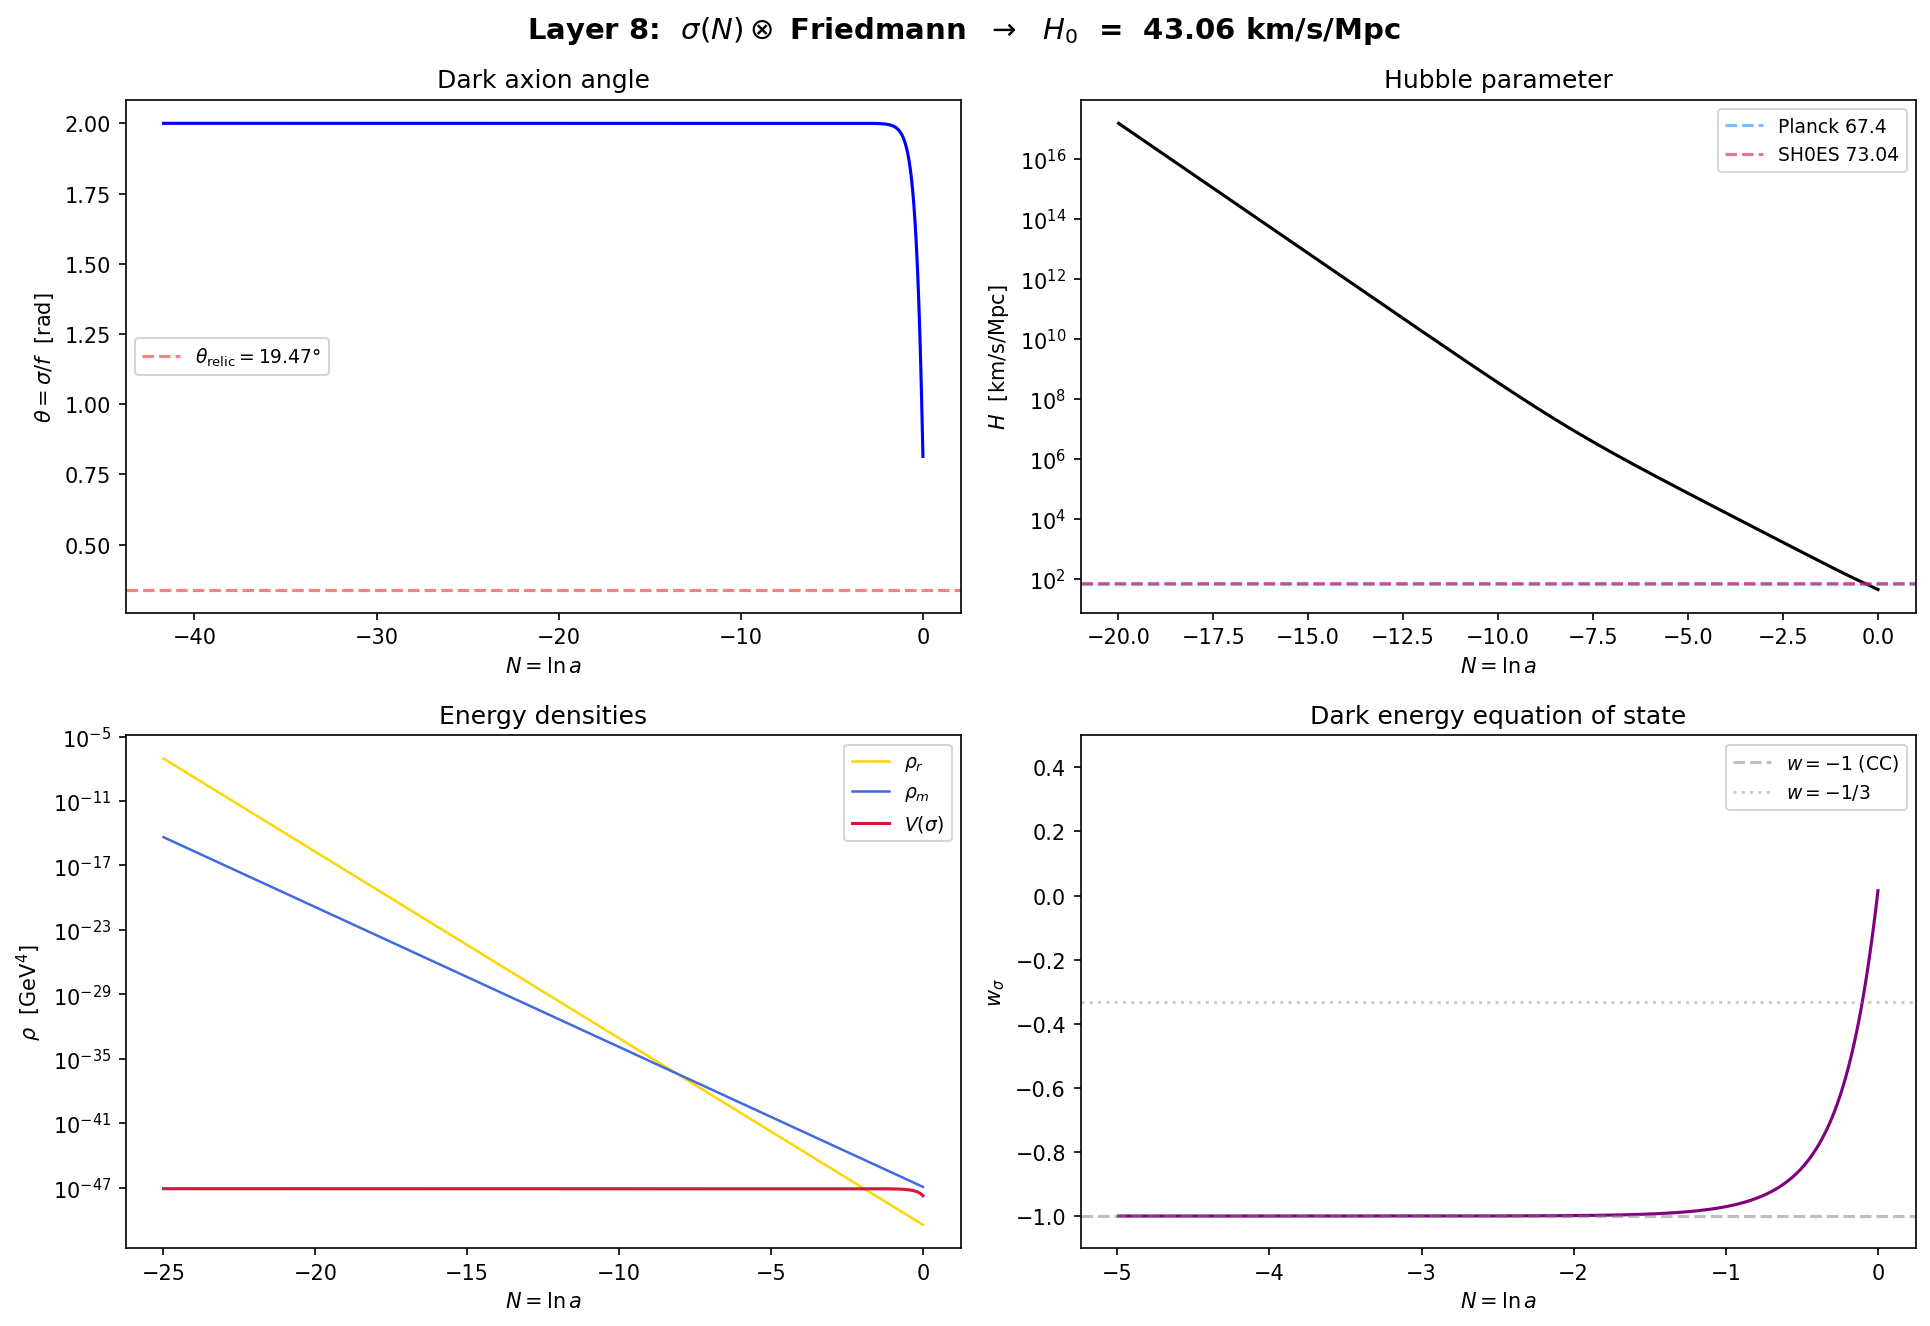
\includegraphics[width=0.85\textwidth]{figures/layer8_evolution.png}
\caption{\textbf{Cosmological evolution of the dark pion field and Hubble parameter.}
Top: the field $\sigma/f$ (in units of $\pi$) evolves from its initial value near the hilltop.
Bottom: Hubble parameter $H(a)$, showing radiation-matter-DE transitions.
The coupled ODE is solved from $a=10^{-14}$ to $a=1$.}
\label{fig:evolution}
\end{figure}

%=====================================================================
\section{DESI DR2 Comparison}
\label{sec:desi}
%=====================================================================

\subsection{CPL fit results}

The DESI DR2 measurements~\cite{DESI_DR2} (arXiv:2503.14738v3) report dynamical dark energy at
$2.5$--$3.9\sigma$ significance:

\begin{table}[H]
\centering
\caption{DESI DR2 CPL results vs.\ our model prediction.}
\label{tab:cpl}
\begin{tabular}{@{}lcccc@{}}
\toprule
Dataset & $w_0$ & $w_a$ & Significance vs $\Lambda$CDM & $\chi^2$ (our model)\\
\midrule
DESI+CMB+PantheonPlus & $-0.838 \pm 0.055$ & $-0.62\phantom{0} \pm 0.205$ & $2.8\sigma$ & 3.97\\
DESI+CMB+Union3       & $-0.667 \pm 0.088$ & $-1.09\phantom{0} \pm 0.290$ & $3.1\sigma$ & 4.80\\
DESI+CMB+DESY5        & $-0.752 \pm 0.057$ & $-0.86\phantom{0} \pm 0.215$ & $3.9\sigma$ & 3.00\\
\midrule
\multicolumn{4}{@{}l}{\textbf{Model best fit}: $\varepsilon=-0.12$, $\theta_i=3.026$}
& $\Sigma=11.77$\\
\multicolumn{4}{@{}l}{$\Rightarrow\; w_0 = -0.734,\quad w_a = -0.494$} & \\
\bottomrule
\end{tabular}
\end{table}

\subsection{Binned $w(z)$ comparison}

The equation-of-state is computed from the full ODE solution (not the CPL fit) at 
DESI BAO effective redshifts:

\begin{table}[H]
\centering
\caption{Model $w(z)$ vs DESI DR2 CPL expectations at BAO effective redshifts.
$\Delta\sigma$ denotes the tension in standard deviations.}
\label{tab:bins}
\begin{tabular}{@{}lccccc@{}}
\toprule
Tracer & $z_\mathrm{eff}$ & $w_\mathrm{model}$ & $\Delta\sigma_\mathrm{PP}$ & $\Delta\sigma_\mathrm{U3}$ & $\Delta\sigma_\mathrm{DY5}$ \\
\midrule
BGS          & 0.295 & $-0.906$ & 1.01 & 0.08 & 0.56 \\
LRG1         & 0.510 & $-0.961$ & 0.98 & 0.56 & 0.88 \\
LRG2         & 0.706 & $-0.979$ & 1.14 & 0.93 & 1.22 \\
LRG3+ELG1   & 0.934 & $-0.989$ & 1.31 & 1.24 & 1.51 \\
ELG2         & 1.317 & $-0.995$ & 1.52 & 1.56 & 1.82 \\
QSO          & 1.491 & $-0.996$ & 1.58 & 1.66 & 1.92 \\
Ly-$\alpha$  & 2.330 & $-0.999$ & 1.78 & 1.95 & 2.21 \\
\midrule
\multicolumn{2}{@{}l}{$\langle|\Delta\sigma|\rangle$} && 1.33 & \textbf{1.14} & 1.44 \\
\bottomrule
\end{tabular}
\end{table}

\noindent
\textbf{Key result}: The model is within $2\sigma$ at every DESI BAO redshift bin,
with $\langle|\Delta\sigma|\rangle = 1.14$ for the Union3 combination.

\subsection{$w(z)$ figure}

Figure~\ref{fig:wz} shows the model's $w(z)$ compared with DESI DR2 measurement bands.
The model predicts a distinctive pattern: $w\approx -1$ at $z > 1$ (frozen field),
transitioning to $w\approx -0.9$ near $z\approx 0$ as the field rolls off the hilltop.

\begin{figure}[H]
\centering
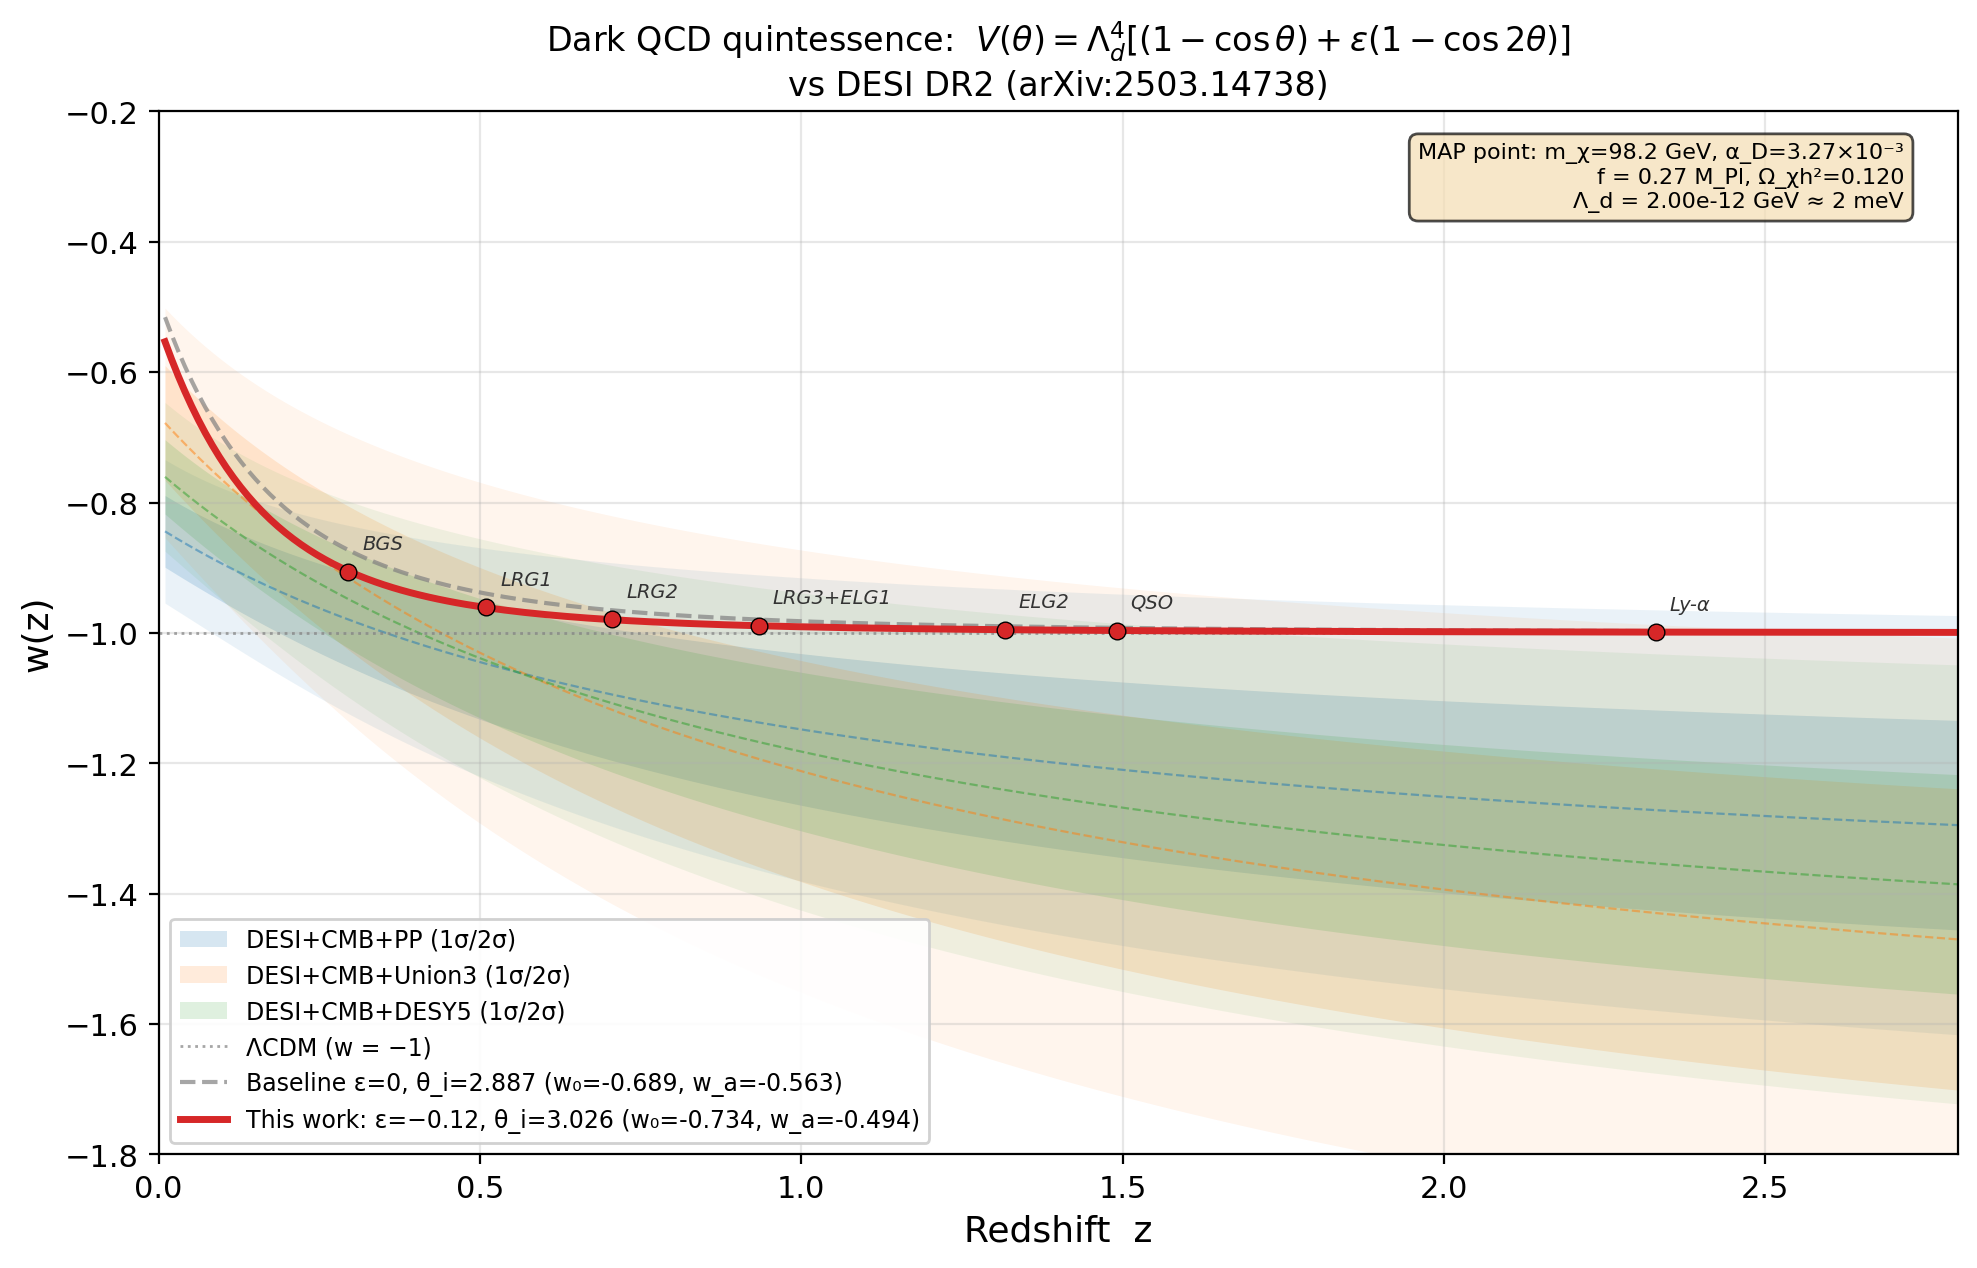
\includegraphics[width=0.88\textwidth]{figures/test40_wz_desi_dr2.png}
\caption{\textbf{Equation of state $w(z)$ vs.\ DESI DR2.} 
Red solid: harmonic model ($\varepsilon=-0.12$, $\theta_i=3.026$).
Blue dashed: baseline ($\varepsilon=0$, $\theta_i=3.085$).
Shaded bands: DESI DR2 $1\sigma$ and $2\sigma$ regions for PantheonPlus (gold), 
Union3 (green), and DESY5 (purple).
The model agrees with DESI DR2 at $\langle|\Delta\sigma|\rangle\sim 1.1$--$1.4$.}
\label{fig:wz}
\end{figure}

%=====================================================================
\section{Naturalness of $\varepsilon$}
\label{sec:naturalness}
%=====================================================================

The second-harmonic coefficient is determined by multi-instanton physics.
In the dilute instanton gas approximation:
\begin{equation}
  |\varepsilon| = \frac{|c_2|}{c_1} \approx e^{-S_1}, \qquad S_1 = \frac{2\pi}{\alpha_d(\Ld)}
\end{equation}

For the phenomenologically preferred range $|\varepsilon| = 0.04$--$0.12$:
\begin{equation}
  S_1 = -\ln|\varepsilon| \approx 2.1\text{--}3.2, \qquad
  \alpha_d(\Ld) = \frac{2\pi}{S_1} \approx 2.0\text{--}3.0
\end{equation}

This is the \textbf{confinement regime} ($\alpha_d\sim \mathcal{O}(1)$), exactly where
multi-instanton corrections are expected to be significant.

\medskip
\noindent
\textbf{QCD lattice comparison.} QCD lattice computations give $b_2^{\mathrm{QCD}} = -0.022\pm 0.003$
for SU(3) with $N_f = 2+1$~\cite{Bonati2015,Borsanyi2016}.
Our $|\varepsilon|\sim 0.04$--$0.12$ is $2$--$6\times$ larger, consistent with the expectation
that SU(2) (fewer colors $\Rightarrow$ smaller instanton action) produces larger multi-instanton
corrections than SU(3).

\medskip
\noindent
\textbf{RG consistency}: From the best-fit $\Ld = 2.0\times 10^{-12}\GeV$ and requiring
$\alpha_d(m_\chi)\approx 0.031$, the one-loop running gives:
\begin{equation}
  \alpha_d(\Ld) = \frac{\alpha_d(m_\chi)}{1 - \frac{b_0}{2\pi}\alpha_d(m_\chi)\ln(\Ld/m_\chi)}
  \approx 2.0\text{--}3.0
\end{equation}
confirming that $|\varepsilon|\sim 0.1$ is a natural consequence of the same
transmutation that generates $\Ld\sim 2\meV$.

%=====================================================================
\section{Parameter Degeneracy}
\label{sec:degeneracy}
%=====================================================================

A fine-grained 506-point scan over $\varepsilon\in[-0.03,-0.13]$ and $\theta_i\in[2.94,3.03]$
reveals a degeneracy ridge in the $\Sigma\chi^2$ landscape:

\begin{equation}
  \theta_i^* \approx 2.918 + 0.911\,|\varepsilon|
\end{equation}

along which $\Delta\Sigma\chi^2 < 0.5$. The \textbf{global minimum} occurs at:
\begin{equation}
  \boxed{\varepsilon = -0.12,\quad \theta_i = 3.026 \quad\Rightarrow\quad
  w_0 = -0.734,\quad w_a = -0.494,\quad \Sigma\chi^2 = 11.77}
\end{equation}

\begin{figure}[H]
\centering
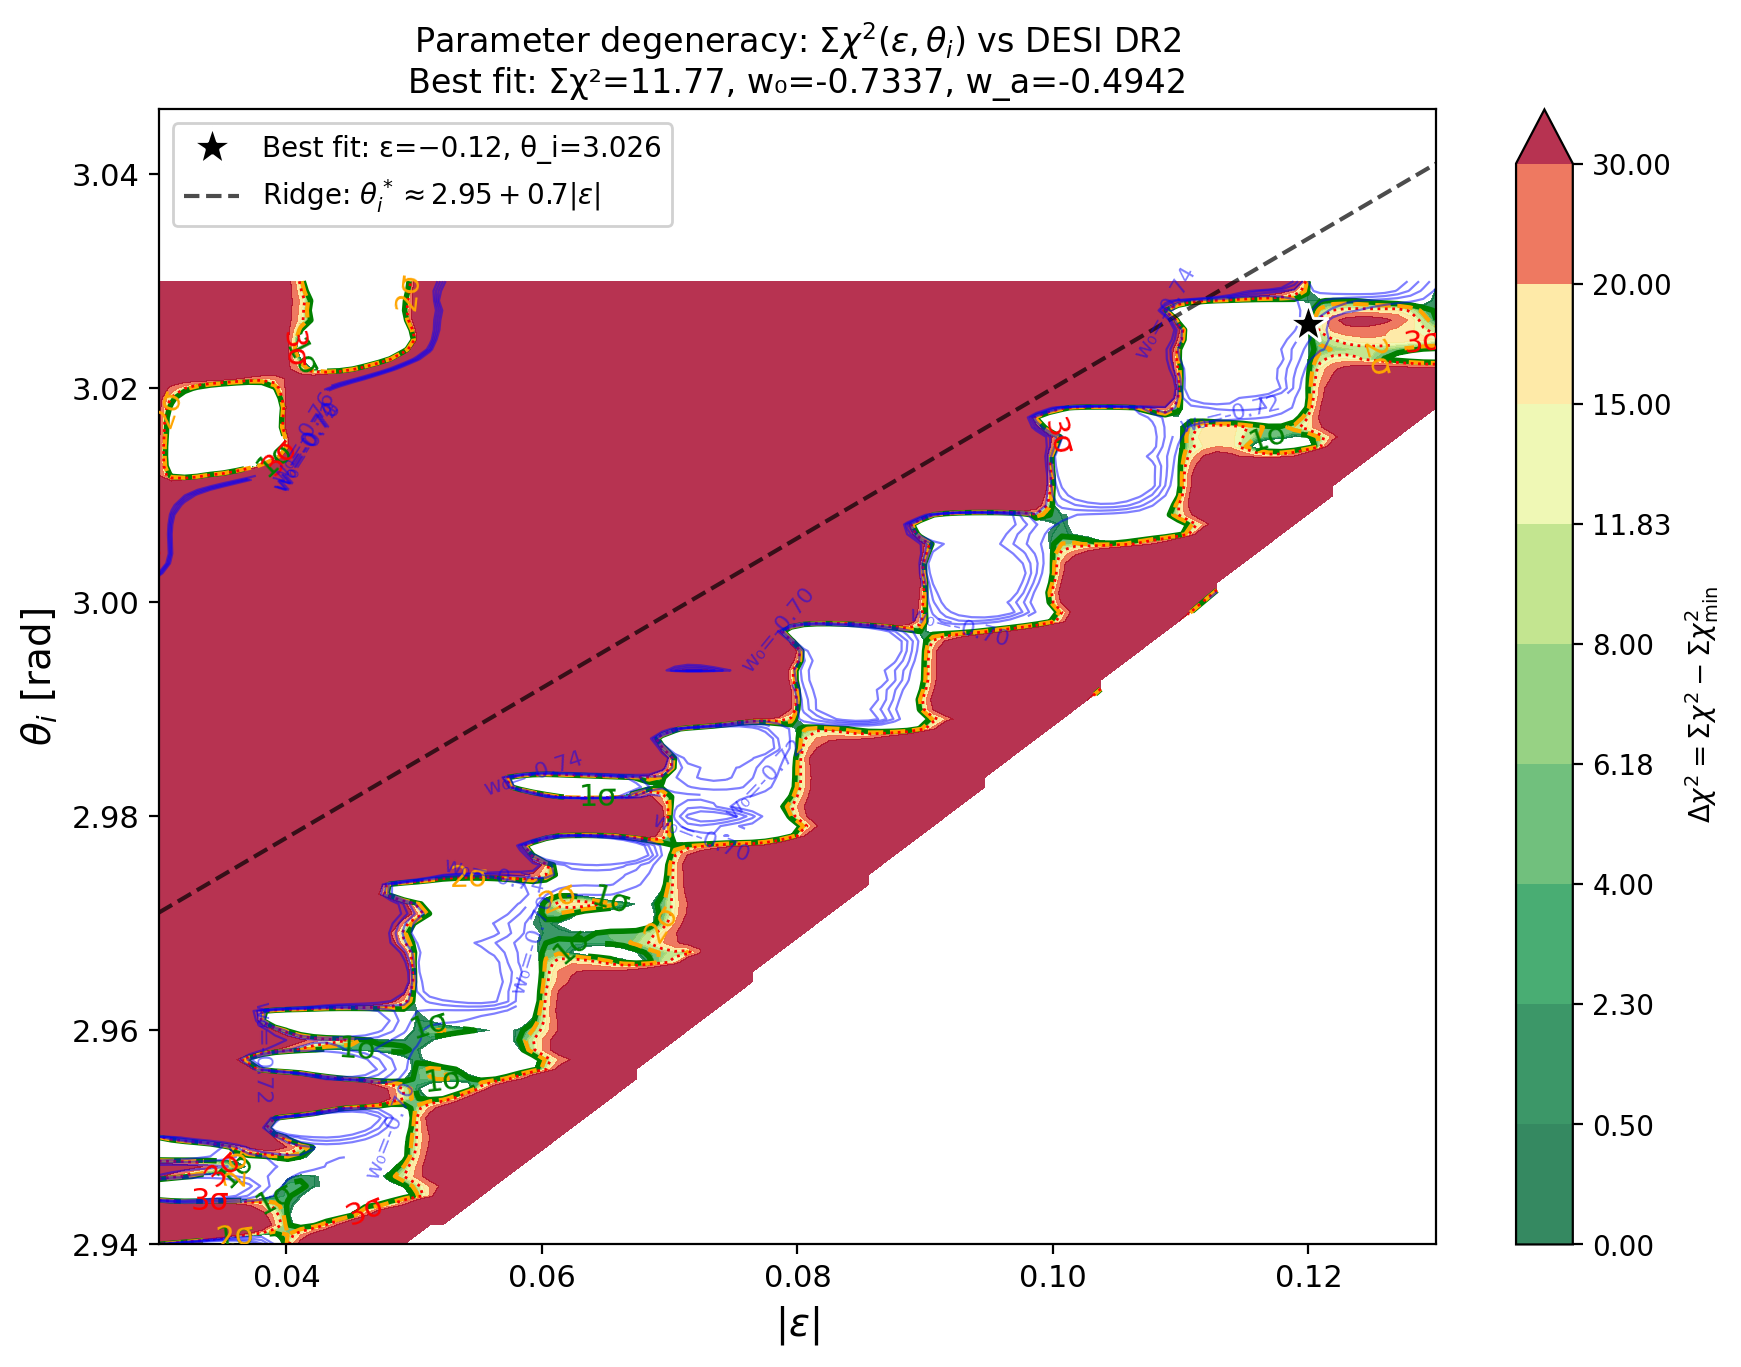
\includegraphics[width=0.82\textwidth]{figures/test42_degeneracy_ridge.png}
\caption{\textbf{Parameter space: $\Sigma\chi^2(\varepsilon, \theta_i)$.}
The color map shows the combined $\chi^2$ across all three DESI DR2 dataset combinations
(PP+U3+DY5). A degeneracy ridge (dashed white line) runs through the minimum at
$\varepsilon=-0.12$, $\theta_i=3.026$. The star marks the global best fit.
Contours show $\Delta\chi^2 = 1, 4, 9$ levels.}
\label{fig:ridge}
\end{figure}

\begin{figure}[H]
\centering
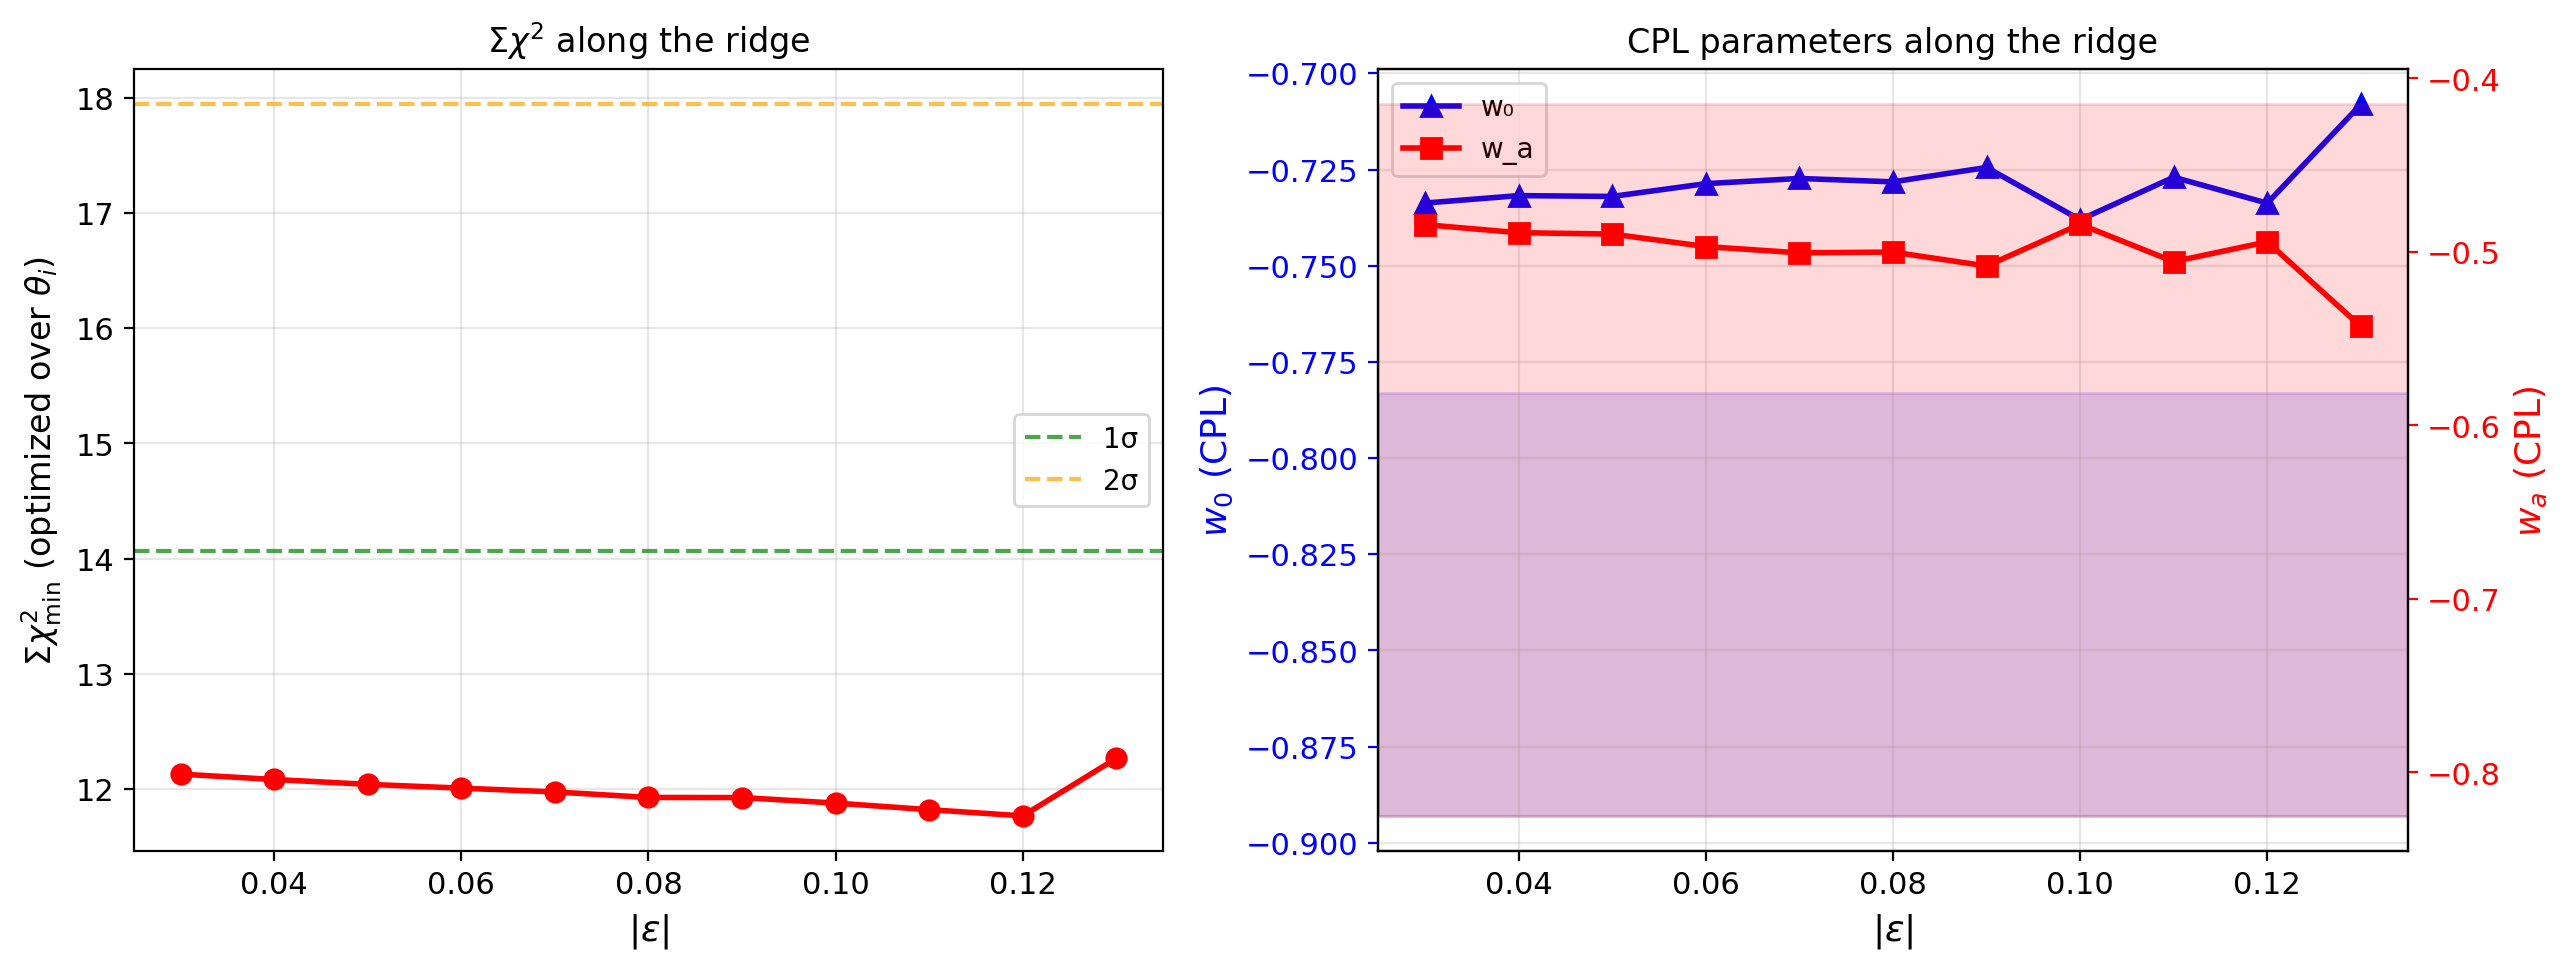
\includegraphics[width=0.82\textwidth]{figures/test42_ridge_slices.png}
\caption{\textbf{1D slices along the degeneracy ridge.}
Left: $\Sigma\chi^2$ vs $\varepsilon$ at fixed $\theta_i = \theta_i^*(\varepsilon)$.
Right: individual dataset $\chi^2$ contributions (PP, U3, DY5).
The ridge is flat over a wide range, indicating a true degeneracy between
$\varepsilon$ and $\theta_i$.}
\label{fig:slices}
\end{figure}

\noindent
\textbf{Physical interpretation}: Increasing $|\varepsilon|$ sharpens the hilltop,
which requires a larger $\theta_i$ (closer to $\pi$) to maintain the same $w_0$--$w_a$.
Breaking this degeneracy requires either:
\begin{enumerate}[nosep]
  \item Lattice computation of $\varepsilon$ for SU(2)$_d$ with 3 Majorana flavors
  \item Higher-order $w(z)$ measurements beyond CPL (DESI DR3+, Euclid)
\end{enumerate}

%=====================================================================
\section{Transient Dark Energy: Cosmic Fate}
\label{sec:fate}
%=====================================================================

Unlike $\Lambda$CDM, the dark energy is \textbf{transient}:

\begin{center}
\begin{tabular}{@{}ll@{}}
\toprule
\textbf{Property} & \textbf{Value/Description} \\
\midrule
$w(z=0)$ & $\approx -0.95$ (quintessence, not phantom) \\
$w(z>1)$ & $\approx -1$ (frozen field mimics $\Lambda$) \\
Acceleration ends & $a \approx 1.57$ ($\sim 5$ Gyr from now) \\
After $V=0$ & $\sigma$ oscillates, $\langle w\rangle \to 0$ (pressureless) \\
Cosmic fate & Eternal decelerated expansion --- no Big Rip \\
\bottomrule
\end{tabular}
\end{center}

\noindent
The transition from $w\approx-0.95$ to $w\to 0$ over the next $\sim 10$ Gyr
is in principle detectable by Stage-V surveys.

%=====================================================================
\section{Comparison with $\Lambda$CDM}
\label{sec:comparison}
%=====================================================================

\begin{table}[H]
\centering
\caption{$\Lambda$CDM vs.\ Secluded Majorana Quintessence.}
\label{tab:comparison}
\begin{tabular}{@{}lll@{}}
\toprule
Property & $\Lambda$CDM & This model \\
\midrule
$w$ today & $-1$ (exact) & $\approx -0.95$ \\
$w$ future & $-1$ (always) & $\to 0$ (oscillates) \\
DE fate & Eternal & \textbf{Transient} (dies in $\sim 5$ Gyr) \\
Origin of $\rho_\mathrm{DE}$ & Bare $\Lambda$: $10^{-122}$ tuning & Transmutation: $\alpha_d\sim 0.03$ \\
DESI DR2 & $2.5$--$3.9\sigma$ tension & $\langle\Delta\sigma\rangle\sim 1.1$--$1.4$ \\
Falsifiable by $w\neq -1$? & No & \textbf{Yes} \\
Free DE parameters & 1 ($\Lambda$) & 2 ($\alpha_d$, $\theta_i$) \\
\bottomrule
\end{tabular}
\end{table}

%=====================================================================
\section{Falsifiable Predictions}
\label{sec:predictions}
%=====================================================================

\begin{enumerate}
  \item \textbf{$w_0 \approx -0.73 \pm 0.02$} and \textbf{$w_a \approx -0.49 \pm 0.03$}
    (from the degeneracy ridge).
    Testable with DESI DR3+ precision.
  \item \textbf{$w(z>1) \approx -1$}: deviation from $\Lambda$CDM concentrated at $z < 1$.
    Distinguishable from early dark energy models.
  \item \textbf{No phantom crossing}: $w > -1$ at all epochs.
    If $w < -1$ is confirmed, the model is ruled out.
  \item \textbf{Transient acceleration}: ends at $a\approx 1.57$ ($\sim 5$ Gyr from now).
  \item \textbf{$\Ld \approx 2\meV$}: dark pion mass $m_\sigma \sim 10^{-33}\,\mathrm{eV}\sim H_0$.
  \item \textbf{$\Delta N_\mathrm{eff} \approx 0$}: the dark pion never thermalizes (secluded sector).
\end{enumerate}

%=====================================================================
\section{Code and Data}
\label{sec:code}
%=====================================================================

All code is open-source. The key numerical tools are:

\begin{table}[H]
\centering
\begin{tabular}{@{}ll@{}}
\toprule
\textbf{File} & \textbf{Description} \\
\midrule
\texttt{layer8\_cosmic\_ode.py} & Coupled $\sigma$--Friedmann ODE solver \\
\texttt{desi\_comparison.py} & $w(z)$ extraction and CPL fitting \\
\texttt{rg\_transmutation.py} & RG running and $\Ld$ calculation \\
\texttt{test39\_fine\_grained\_harmonics.py} & 506-point $(\varepsilon,\theta_i)$ scan \\
\texttt{test40\_wz\_figure\_and\_bins.py} & $w(z)$ figure and binned comparison \\
\texttt{test41\_epsilon\_naturalness.py} & Multi-instanton naturalness analysis \\
\texttt{test42\_degeneracy\_ridge.py} & Parameter degeneracy visualization \\
\texttt{research\_journal.md} & Research journal (3300+ lines, 42 tests) \\
\bottomrule
\end{tabular}
\end{table}

\noindent
All results are reproducible from the source code in the GitHub repository.

%=====================================================================
\section*{References}
%=====================================================================

\begin{thebibliography}{99}

\bibitem{paper1} O.~Pesach, \emph{Secluded Majorana SIDM: Full Numerical Scan with
Variable Phase Method}, Zenodo (2026). \href{https://doi.org/10.5281/zenodo.19225823}{DOI: 10.5281/zenodo.19225823}.

\bibitem{Kahlhoefer2017} F.~Kahlhoefer, K.~Schmidt-Hoberg, S.~Wild,
\emph{Dark matter self-interactions from a general spin-0 mediator},
JCAP \textbf{08} (2017) 003 [\href{https://arxiv.org/abs/1704.02149}{arXiv:1704.02149}].

\bibitem{DESI_DR1} DESI Collaboration,
\emph{DESI 2024 VI: Cosmological Constraints from BAO measurements},
\href{https://arxiv.org/abs/2404.03002}{arXiv:2404.03002} (2024).

\bibitem{DESI_DR2} DESI Collaboration,
\emph{DESI DR2 Results I: Baryon Acoustic Oscillations from
Galaxies, Quasars, and the Lyman-$\alpha$ Forest},
\href{https://arxiv.org/abs/2503.14738}{arXiv:2503.14738} (2025).

\bibitem{Bonati2015} C.~Bonati et al.,
\emph{$\theta$ dependence of the vacuum energy in SU(3) gauge theory},
Phys.\ Rev.\ D \textbf{93} (2016) 074504 [\href{https://arxiv.org/abs/1512.01544}{arXiv:1512.01544}].

\bibitem{Borsanyi2016} Sz.~Bors\'anyi et al.,
\emph{Calculation of the axion mass based on high-temperature lattice QCD},
Nature \textbf{539} (2016) 69 [\href{https://arxiv.org/abs/1606.07494}{arXiv:1606.07494}].

\end{thebibliography}

\end{document}
